\documentclass[letterpaper,12pt]{article}
\usepackage{tabularx} % extra features for tabular environment
\usepackage{amsmath}  % improve math presentation
\usepackage{float}
\usepackage{pdfpages}

\usepackage{graphicx} % takes care of graphic including machinery
\graphicspath{ {./figures/} }
\usepackage[margin=1in,letterpaper]{geometry} % decreases margins
\usepackage{cite} % takes care of citations
\usepackage[final]{hyperref} % adds hyper links inside the generated pdf file
\hypersetup{
	colorlinks=true,       % false: boxed links; true: colored links
	linkcolor=blue,        % color of internal links
	citecolor=blue,        % color of links to bibliography
	filecolor=magenta,     % color of file links
	urlcolor =blue         
}




\begin{document}

\title{Experiment 1 Preliminary Work \protect\\ Diodes and Rectifiers}
\author{Ahmet Akman 2442366 \protect\\}
\date{\today}
\maketitle
\tableofcontents
%\begin{abstract}
%abstract
%\end{abstract}

%\section{Introduction}
In this document the actions corresponding requirements defined in the Experiment Manual are  represented.
\section{Step 1}
Notes on signal generators, oscilloscopes and multimeters are studied and reviewed the fundamentals.
\section{Step 2}
Notes on dioedes document is studied. The datasheets of the diodes to be used in this experiment are reviewed, which are \href{https://www.vishay.com/docs/88503/1n4001.pdf}{1N40007} , \href{https://www.vishay.com/docs/88536/ba157.pdf}{BA159} ,\href{https://logosfoundation.org/elektron/mixers/AA119.pdf}{AA119} ,and \href{https://www.vishay.com/docs/85604/bzx55.pdf}{BZX55C-6V2}.   
\section{Step 3}
%MATLAB and Latex
In this step characteristics of linear modeled junction diodes are analyzed according to the I vs V equation as follows,
\[
I  = I_s[e^\frac{qV}{nkT} - 1]    
\] 
Ideality constant n is taken 1 for both cases. From explanation in the manual \(\frac{kT}{q}\) is taken as 25 mV at temperature (20\(\circ\)C ) . The common pievewise linear model for a junction diode is given in Figure 1.
\begin{figure}[H]
    \centering
   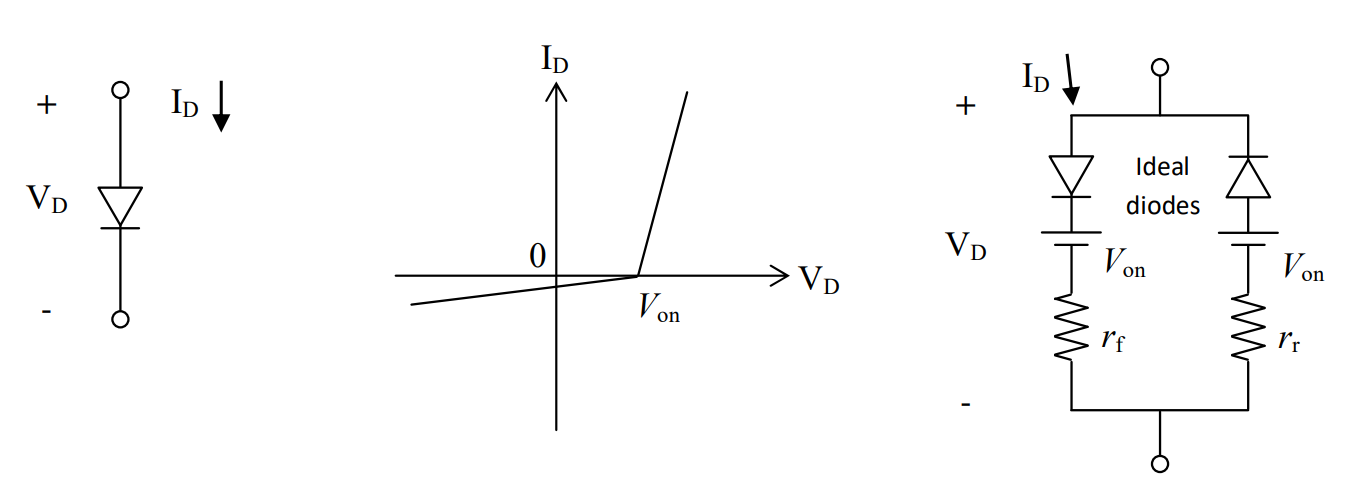
\includegraphics[width=1\textwidth]{3_1.png}
   \caption{Common piecewise linear model for a junction diode.}
\end{figure} 

\subsection{a)}
In table 1 the i-v values for the given voltages are obtained by taking the reverse saturation value 2.5xE-7 . The results are calculated using MATLAB.

\begin{table}[H]
\begin{center}
\caption{ I vs V}
\vspace{2mm}
\begin{tabular}{||c | c ||} 
\hline
V(Volts) & I (Amps) \\ [0.5ex] 
\hline\hline
-0.40 & -2.499999718662063e-07  \\ 
\hline
-0.20 & -2.499161343430244e-07  \\ 
\hline
0 & 0  \\ 
\hline
0.10 & 1.339953750828606e-05  \\ 
\hline
0.20 & 7.449894967604320e-04  \\ 
\hline
0.30 & 0.040688447854751  \\ 
\hline
0.40 & 2.221527380126968  \\ 
\hline
\end{tabular}
\end{center}
\end{table}
Then the i versus v plot is obtained ,and given in Figure 2.

\begin{figure}[H]
\centering
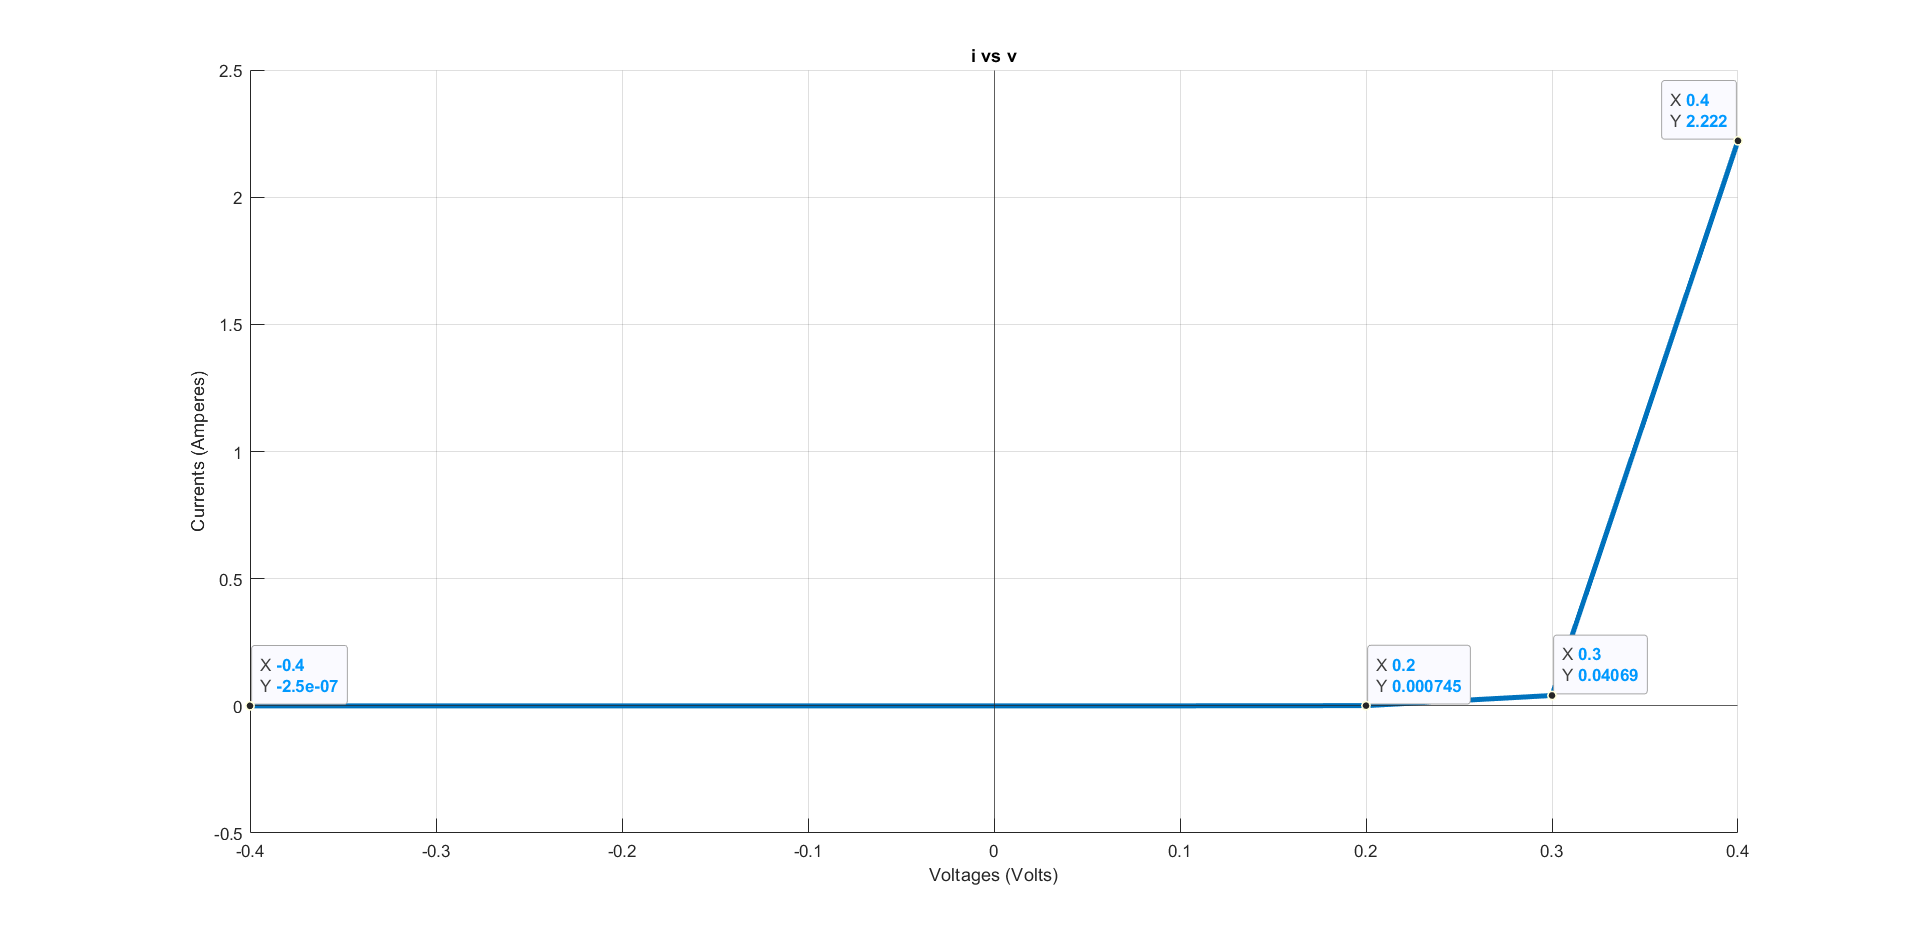
\includegraphics[width=1\textwidth]{3a.png}
\caption{i versus v plot}
\end{figure} 
    
\begin{table}[H]
    \begin{center}
    \caption{ Parameters obtained from the plot}
    \vspace{2mm}
    \begin{tabular}{||c | c | c ||} 
    \hline
    \(V_{on}\) &  \(r_f\) & \(r_r\)\\ [0.5ex] 
    \hline\hline
    0.3V & 0.046\(\Omega\)  & 2.5\(\Omega\)   \\ 
    
\hline
\end{tabular}
\end{center}
\end{table}
    
So the piecewise linear model parameters are determined ,and provided in Table 2.

    
    
\subsection{b)}
In table 3 the i-v values for the given voltages are obtained by taking the reverse saturation value 1E-15 . The results are calculated using MATLAB.

\begin{table}[H]
\begin{center}
\caption{ I vs V}
\vspace{2mm}
\begin{tabular}{||c | c ||} 
\hline
V(Volts) & I (Amps) \\ [0.5ex] 
\hline\hline
-0.40 & -9.999998874648254e-16  \\ 
\hline
-0.20 & -9.996645373720976e-16  \\ 
\hline
0 & 0  \\ 
\hline
0.20 & 2.979957987041728e-12  \\ 
\hline
0.40 & 8.886109520507873e-09  \\ 

\hline
0.50 & 4.851651944097903e-07  \\ 
\hline
0.60 & 2.648912212884338e-05  \\ 
\hline
0.70 & 0.001446257064290  \\ 
\hline
0.80 & 0.078962960182680  \\ 
\hline
\end{tabular}
\end{center}
\end{table}

Then the i versus v plot is obtained ,and given in Figure 2.


\begin{figure}[H]
    \centering
    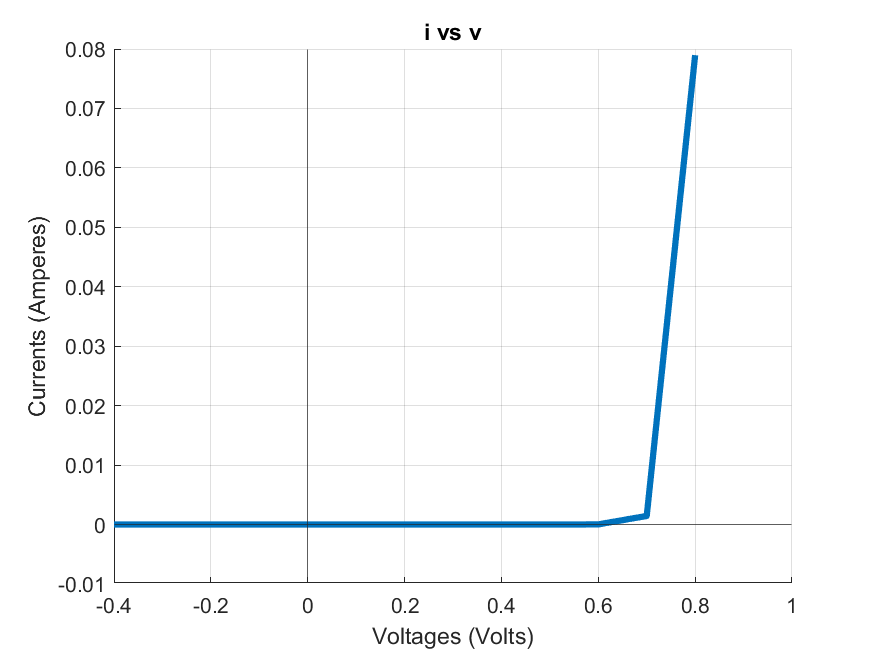
\includegraphics[width=1\textwidth]{3b.png}
    \caption{i versus v plot}
\end{figure} 
\begin{table}[H]
    \begin{center}
    \caption{ Parameters obtained from the plot}
    \vspace{2mm}
    \begin{tabular}{||c | c | c ||} 
    \hline
    \(V_{on}\) &  \(r_f\) & \(r_r\)\\ [0.5ex] 
    \hline\hline
    0.7V & 1.2893\(\Omega\)  & 68.97\(\Omega\)   \\ 
    
\hline
\end{tabular}
\end{center}
\end{table}
So the piecewise linear model parameters are determined ,and provided in Table 2.

\section{Step 4}

%Hand

A practical half-wave rectifier circuit schematic taken as reference ,and given in Figure 4.
\begin{figure}[H]
    \centering
   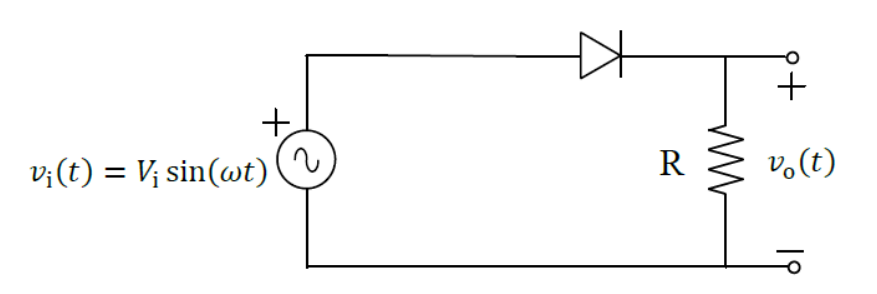
\includegraphics[width=1\textwidth]{4_1.png}
   \caption{Half-wave circuit schematic for the Step 4}
\end{figure} 
Then the following analysis ,given in Figure 5, is made on paper with the required sketch. 

\begin{figure}[H]
    \centering
   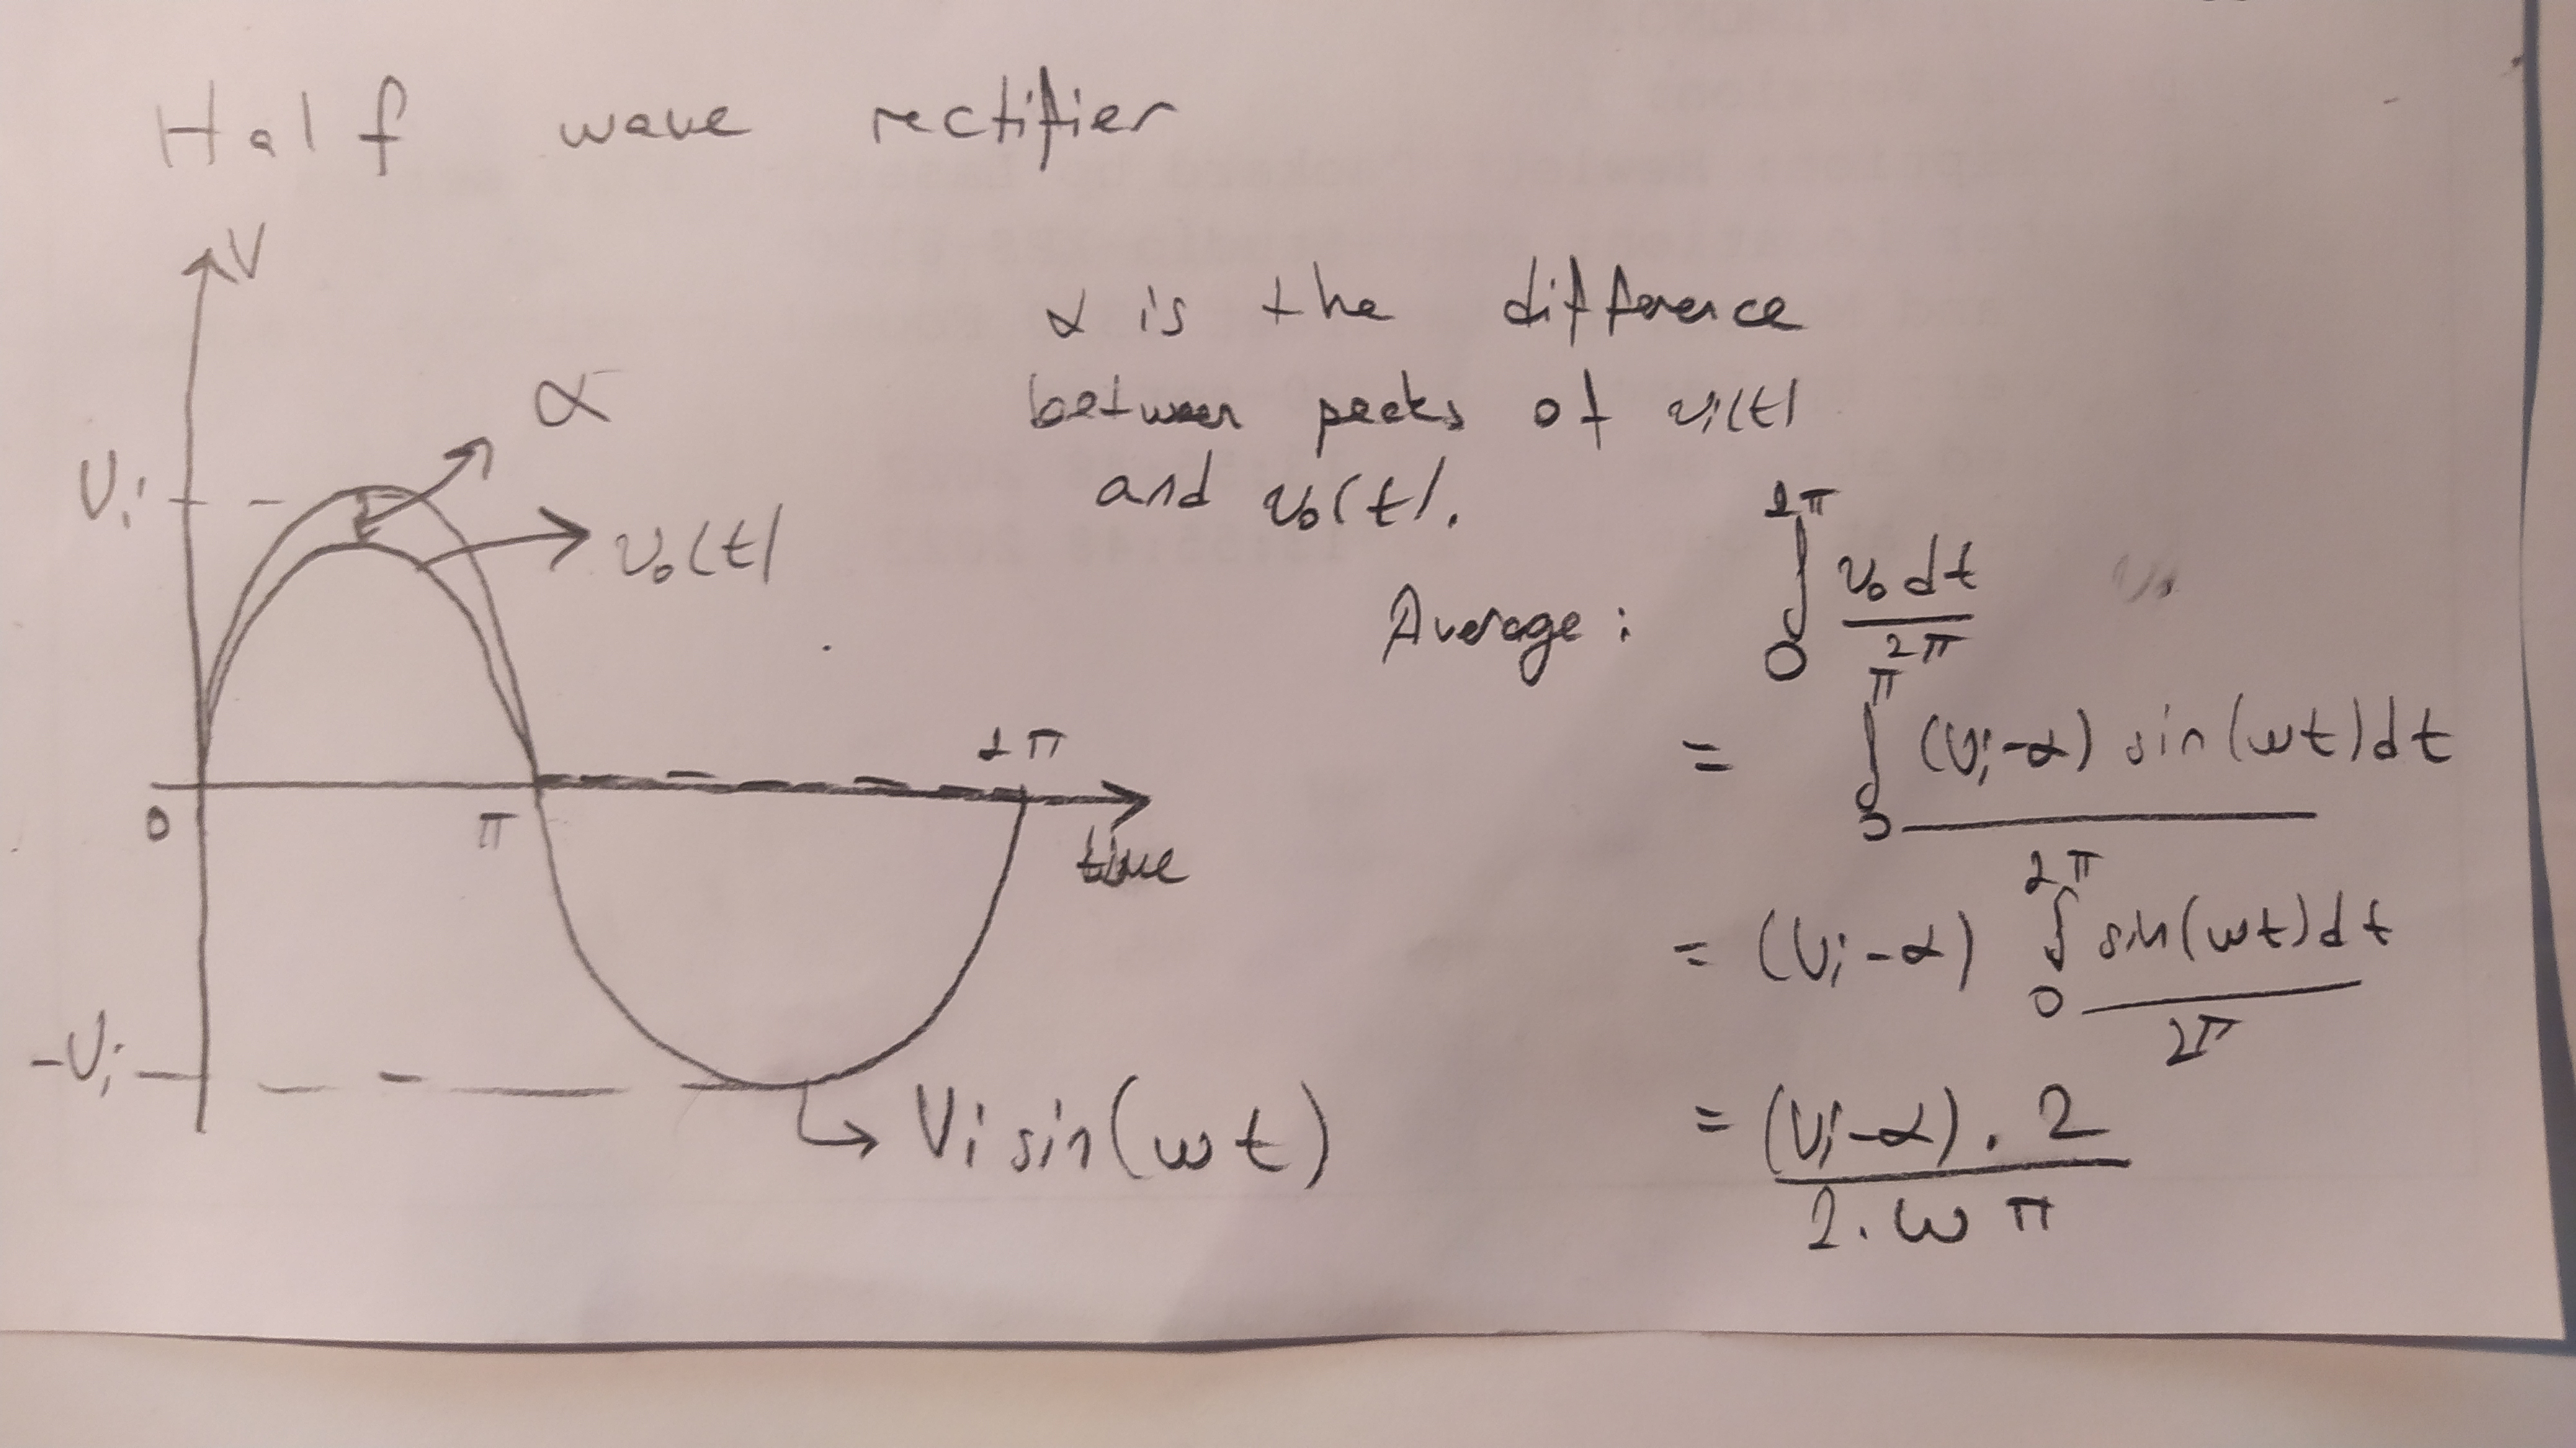
\includegraphics[width=1\textwidth]{Q4.jpg}
   \caption{Half-wave circuit analysis for the Step 4}
\end{figure} 
Here , \(\alpha\) denotes the difference between the peaks of the \(v_o\) and \(v_i\) which is resulted from the forward resistance of the diode.
So ;
\[
    \alpha = V_i* \frac{r_f}{r_f + R }     
\]
The derived expression for the average voltage is given in the Figure 5. The assumption is made that backward resistance is negligible.
\section{Step 5}
%Hand
 In step 5 the diode clamper circuit is analyzed. The circuit schematic given in Figure 6 is taken as the reference.

\begin{figure}[H]
    \centering
   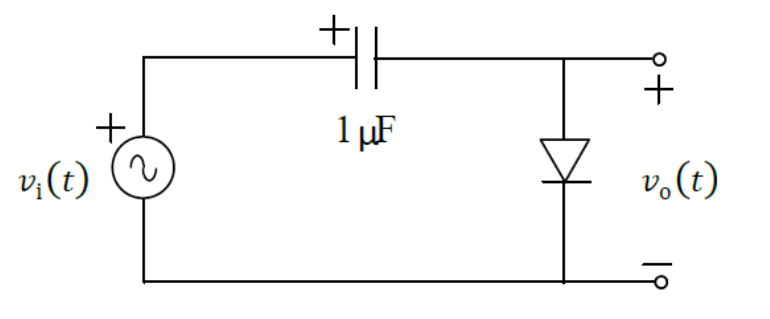
\includegraphics[width=1\textwidth]{5_1.png}
   \caption{Diode clamper circuit schematic for the Step 5}
\end{figure} 
Then the circuit presented in Figure 7 is constructed in LTSpice environment.
\begin{figure}[H]
    \centering
   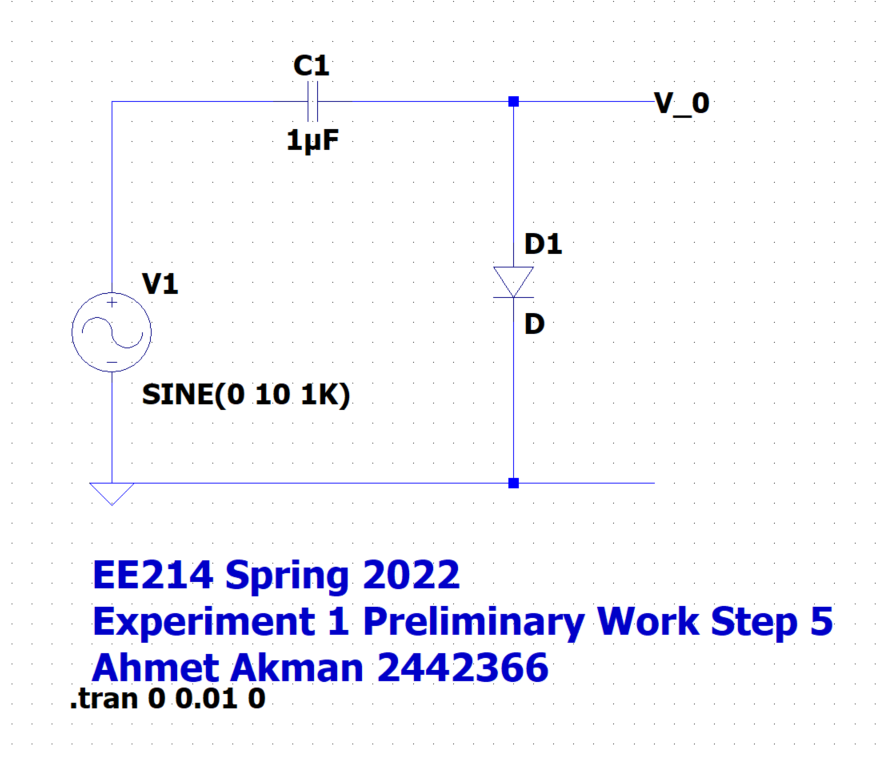
\includegraphics[width=1\textwidth]{5SCH.png}
   \caption{Diode clamper circuit simulation schematic for the Step 5}
\end{figure} 



\subsection{a)}
First, the input is adjusted as a sine wave with amplitude 10 Volts. Then the plot given in Figure 8 is obtained.
\begin{figure}[H]
    \centering
   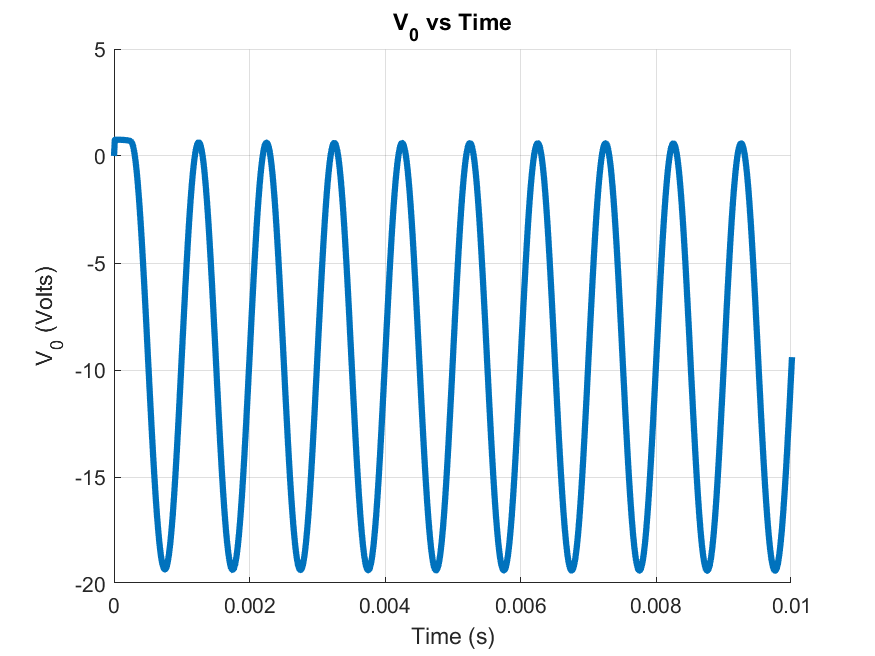
\includegraphics[width=1\textwidth]{5a.png}
   \caption{Diode clamper circuit simulation plot}
\end{figure} 
As it can be observed the average value of the voltage across diode is appriximately -10 Volts.
\subsection{b)}
Secondly, the input is adjusted as a square wave with 10 Volts. Then the plot given in Figure 9 is obtained.

\begin{figure}[H]
    \centering
   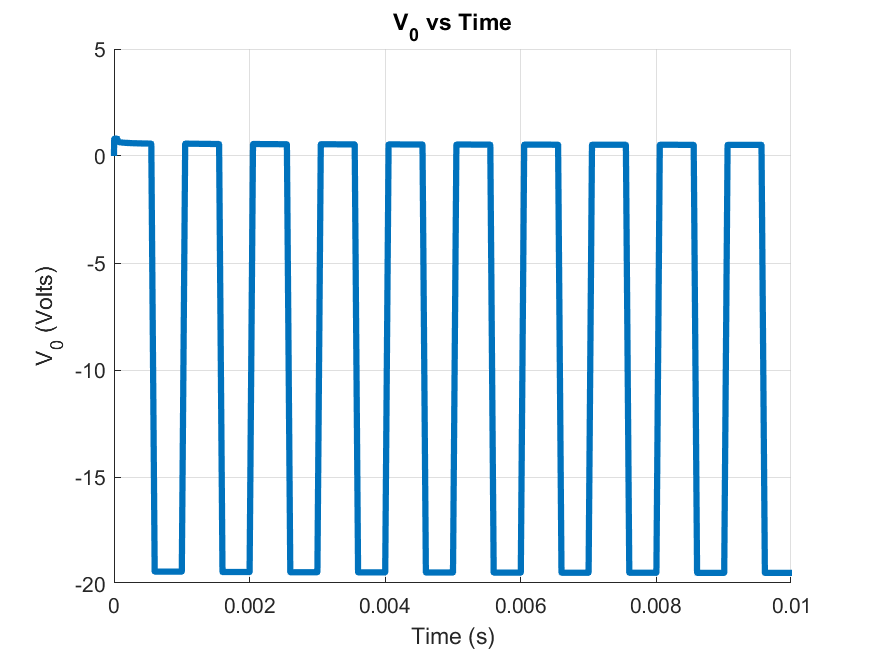
\includegraphics[width=1\textwidth]{5b.png}
   \caption{Diode clamper circuit simulation plot (Square wave input)}
\end{figure} 
As it can be observed the average value of the voltage across diode is appriximately -10 Volts. 

\section{Step 6}
For step 6 , the half wave rectifier circuit with a capacitive load is used the reference circuit is given in Figure 10. Also note that the plots wanted in the summary are given in Appendix B  ( \pageref{AB} ).
\begin{figure}[H]
    \centering
   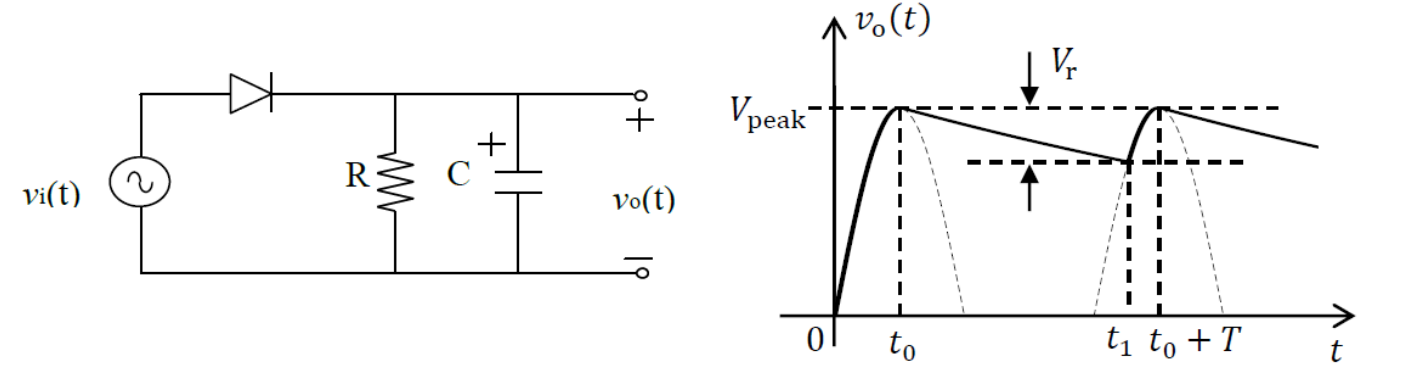
\includegraphics[width=1\textwidth]{6_1.png}
   \caption{Half-wave rectifier circuit schematic for the Step 6}
\end{figure} 
The simulate the circuit the structure in Figure 11 is constructed in LTSpice environment.

\begin{figure}[H]
    \centering
   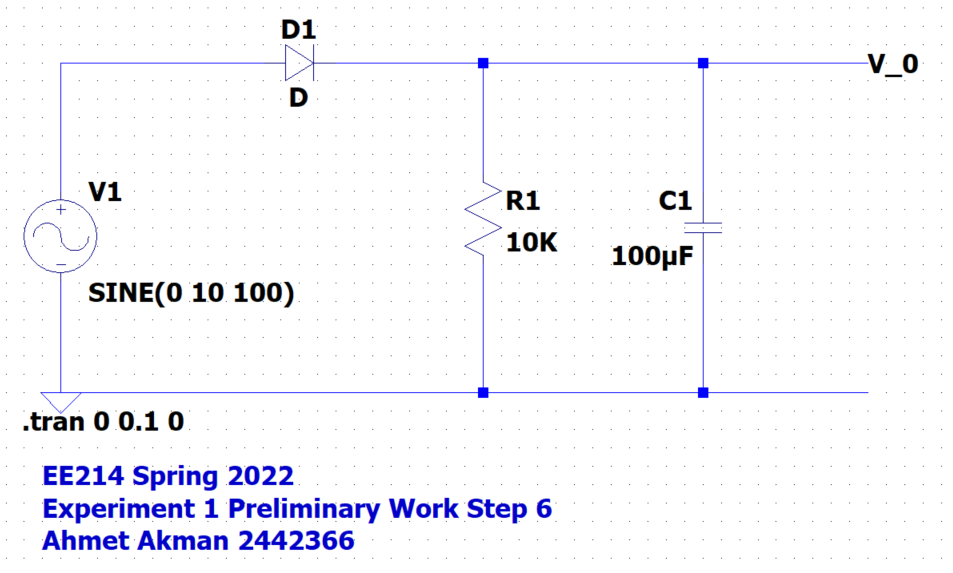
\includegraphics[width=1\textwidth]{6SCH.png}
   \caption{Half-wave rectifier circuit simulation schematic for the Step 6}
\end{figure} 



\subsection{a)}
Here it is expected to find the value of Resistor which makes \(V_r\) value less than the 1 percent of the output voltage. Since output voltage can be approximated as equal to the input voltage, the deviation is needed to be in 0.1 Volts range. So, if the R value is selected as 1k\(\Omega\)  the requirement is barely become satisfied. 

\subsection{b)}
As a result of the simulation work, the plot in Figure 12 is obtained.
\begin{figure}[H]
    \centering
   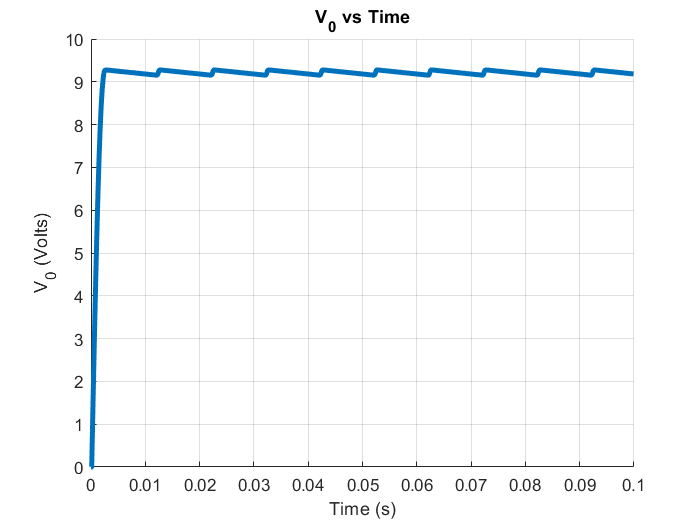
\includegraphics[width=1\textwidth]{6.png}
   \caption{Half wave rectifier circuit simulation plot \(V_o\) }
\end{figure} 



\subsection{c)}
%%%% TODO TODO TODO TODO
As done in the Step 4, it can be said that \(V_r\) become equal to the \(V_{peak}\) . Also by the calculations mentioned in the Step 4 (assuming diode is ideal) \(V_{DC}\) becomes \[V_{DC} = \frac{1}{20 \pi^2}\]
\section{Step 7}
In step 7 the full-wave rectifier circuit is simulated according to the circuit schematic given in Figure 13.

\begin{figure}[H]
    \centering
   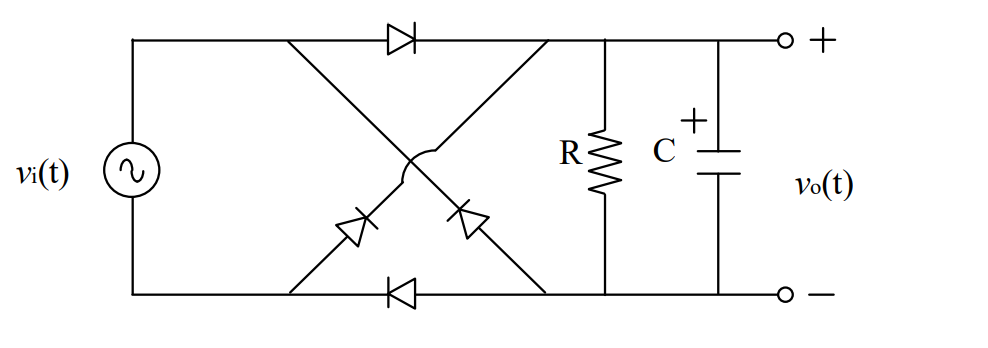
\includegraphics[width=1\textwidth]{7_1.png}
   \caption{Full-wave rectifier circuit schematic for the Step 7}
\end{figure} 
Then  the circuit in Figure 14 is set in  LTSpice environment.

\begin{figure}[H]
    \centering
   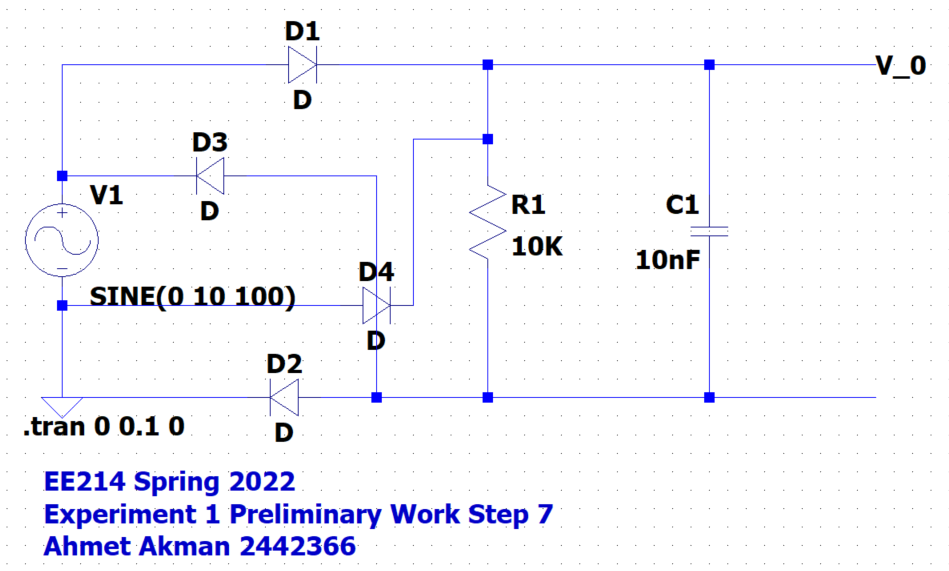
\includegraphics[width=1\textwidth]{7SCH.png}
   \caption{Full-wave rectifier circuit simulation schematic for the Step 7}
\end{figure} 
The capacitive load is set to different loads. For the case of no capacitive load the plot in Figure 15 is observed.  
\begin{figure}[H]
    \centering
   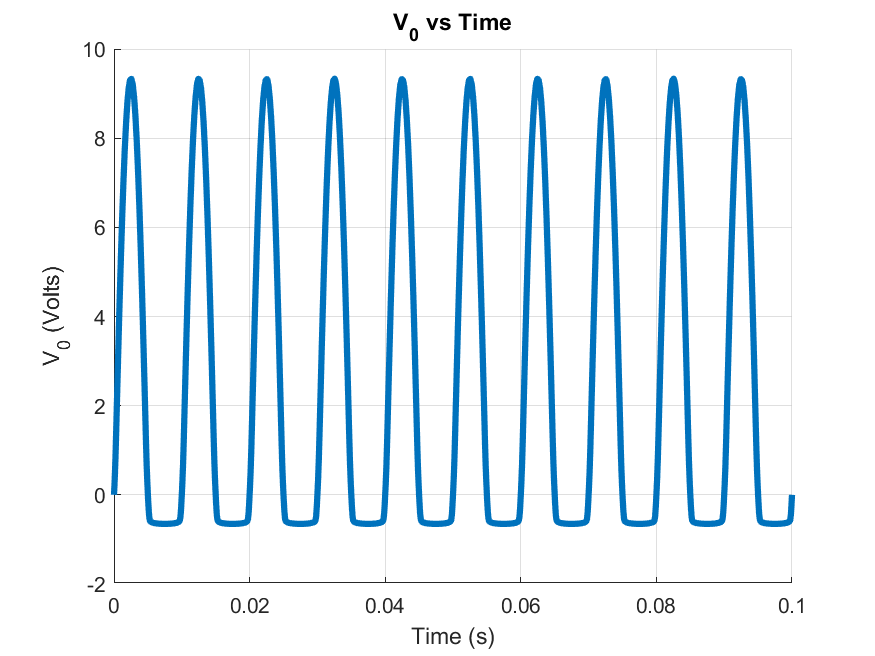
\includegraphics[width=1\textwidth]{7_empty.png}
   \caption{Full-wave rectifier circuit simulation plot \(V_o\) || no capacitor }
\end{figure} 
For the case of 10nF capacitive load the plot in Figure 16 is observed.

\begin{figure}[H]
    \centering
   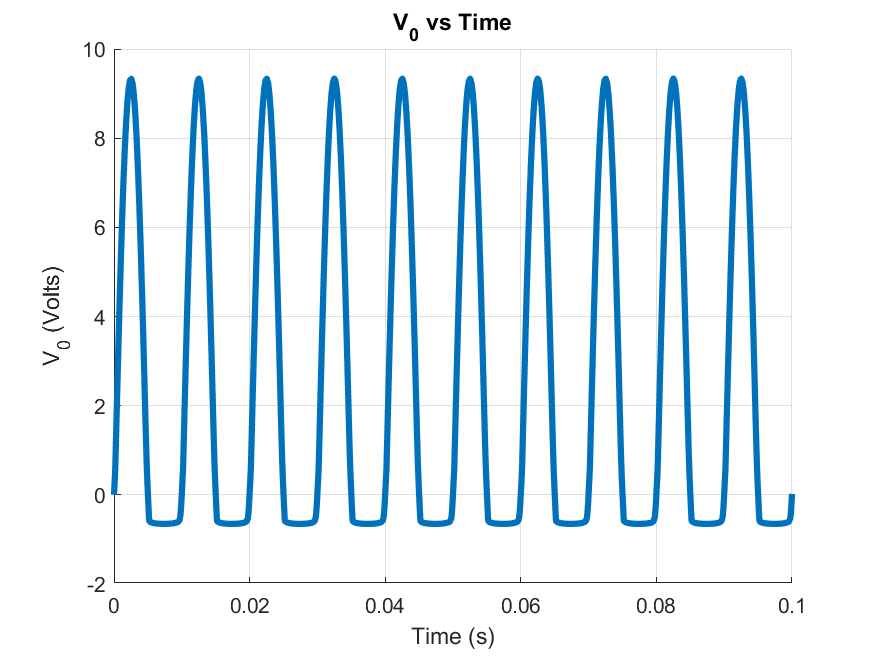
\includegraphics[width=1\textwidth]{7_10nF.png}
   \caption{Full-wave rectifier circuit simulation plot \(V_o\) || 10nF capacitor}
\end{figure} 

Lastly the plot in Figure 17 is obtained for the capacitive load of 1uF.

\begin{figure}[H]
    \centering
   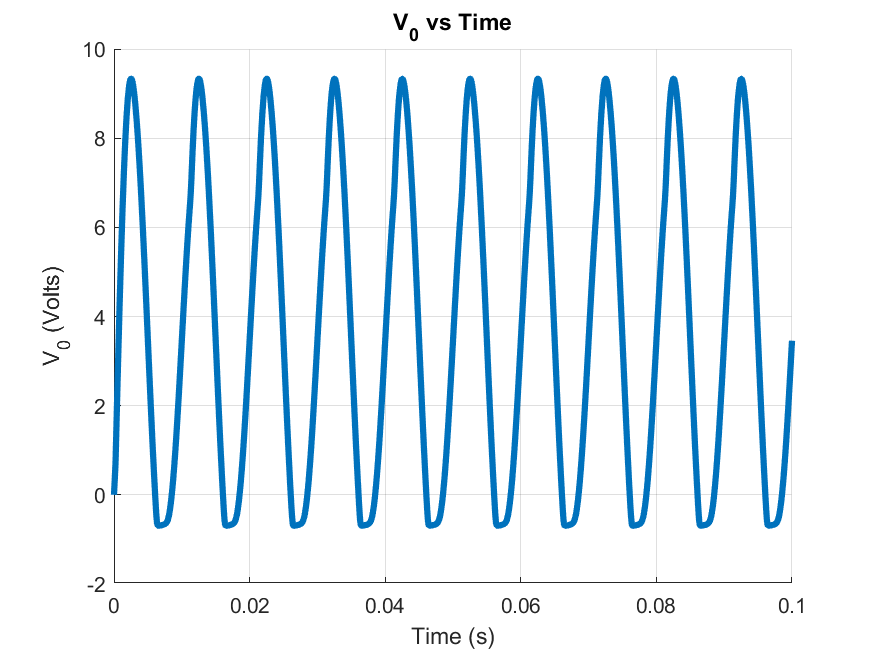
\includegraphics[width=1\textwidth]{7_1uF.png}
   \caption{Full-wave rectifier circuit simulation plot \(V_o\) || 1uF capacitor }
\end{figure} 

To sum up , following comments can be made. While there is a slight difference between the cases of not having capacitor and 10nF capacitor, the case of 10uF capacitor shows a significant compansation.


\section{Step 8}
%LTSpice
In this step the piecewise linear model of the zener diodes are investigated. A common piecewise linear model for a zener diode is presented in Figure 18.

\begin{figure}[H]
    \centering
   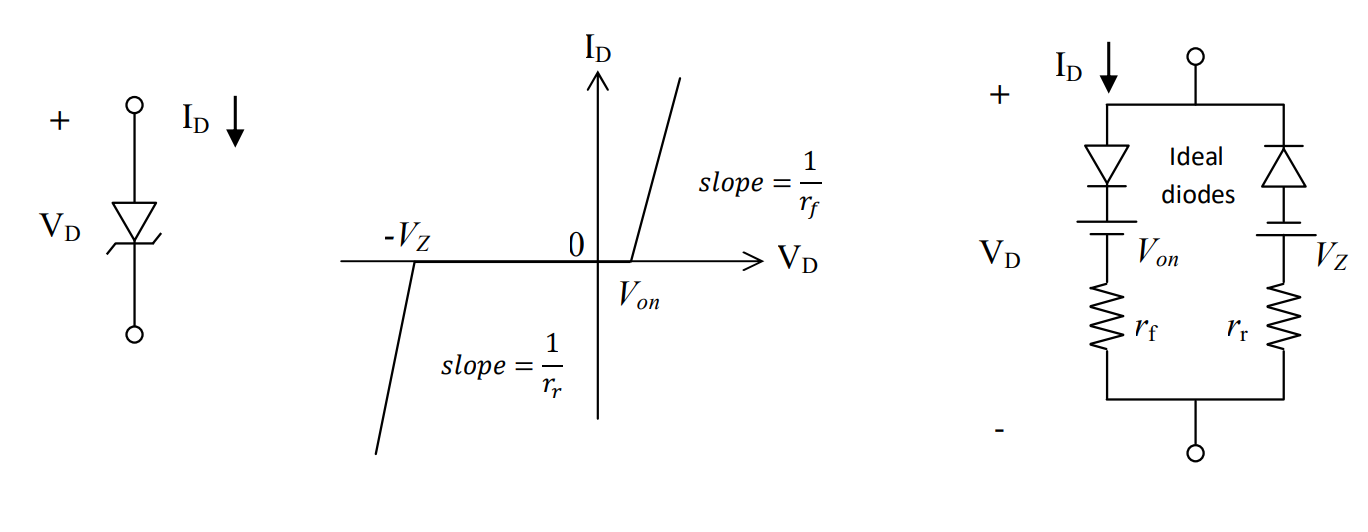
\includegraphics[width=1\textwidth]{8_1.png}
   \caption{Common piecewise linear model for a zener diode.}
\end{figure} 

As being mentioned in the step 2 ,  parameters presented in Table 5 are obtained from the datasheet of zener diode \href{https://www.vishay.com/docs/85604/bzx55.pdf}{BZX55C-6V2} . 
\begin{table}[H]
    \begin{center}
    \caption{ Parameters from datasheet}
    \vspace{2mm}
    \begin{tabular}{||c | c ||} 
    \hline
    Parameter & Value \\ [0.5ex] 
    \hline\hline
    \(V_{on}\) & 0.5V  \\ 
    \hline
    \(V_z\) & 6.2V  \\ 
    \hline
    \(r_f\) & 0.003 \(\Omega\)  \\ 
    \hline
    \(r_r\)& 1 to 10 \(\Omega\)  \\ 
\hline
\end{tabular}
\end{center}
\end{table}


\section{Step 9}
%LTSpice
For step 9 DC level shifter circuit given in Figure 19 is investigated. 
\begin{figure}[H]
    \centering
   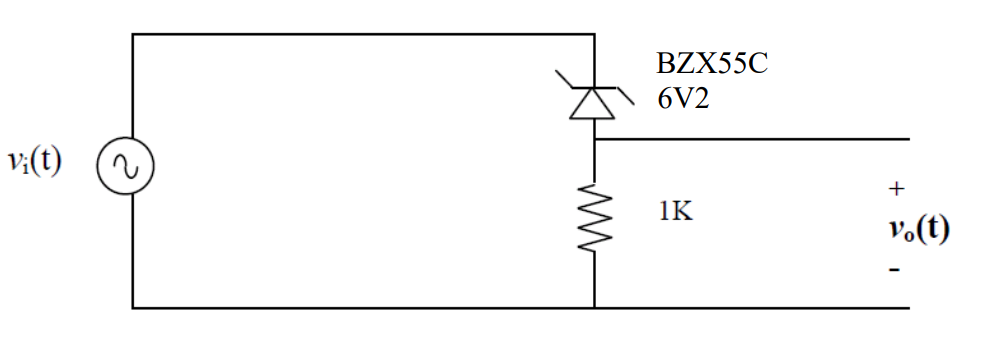
\includegraphics[width=1\textwidth]{9_1.png}
   \caption{DC level shifter circuit schematic for the Step 9}
\end{figure} 
The circuit given in Figure 20 is constructed in LTSpice environment.

\begin{figure}[H]
    \centering
   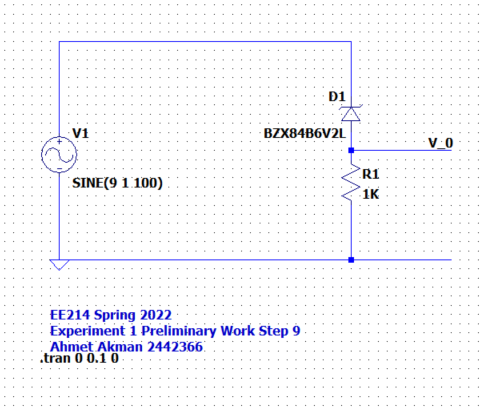
\includegraphics[width=1\textwidth]{9SCH.png}
   \caption{DC level shifter circuit simulation schematic for the Step 9}
\end{figure} 
As the result the plot given in Figure 21 is obtained.

\begin{figure}[H]
    \centering
   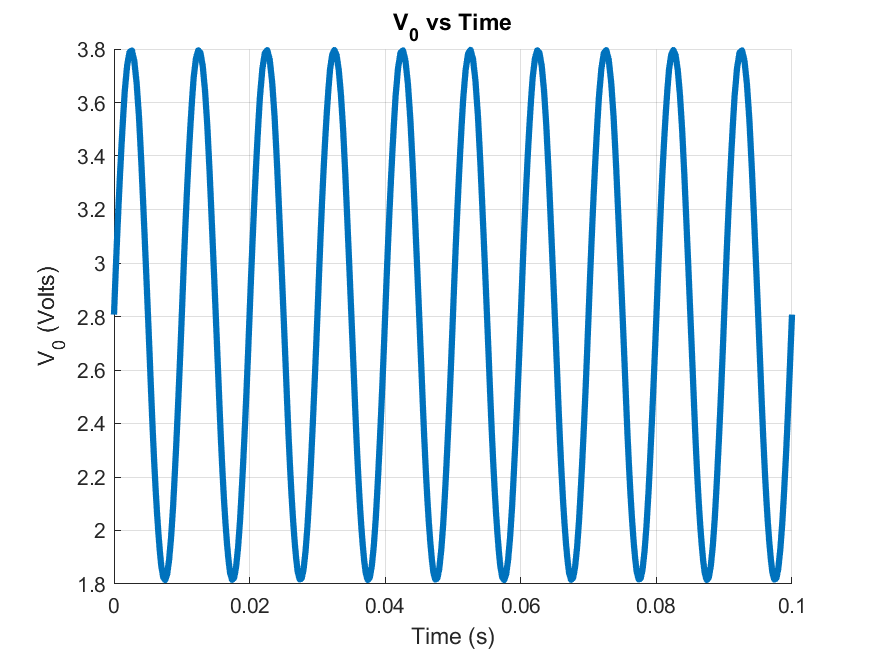
\includegraphics[width=1\textwidth]{9.png}
   \caption{DC level shifter circuit simulation  plot \(V_o\)}
\end{figure} 
It can be said that the input is shifted appriximately 6 Volts.
\section{Step 10}
%LTSpice
For the steo 10 the circuit given in Figure 22 is taken as a reference.
\begin{figure}[H]
    \centering
   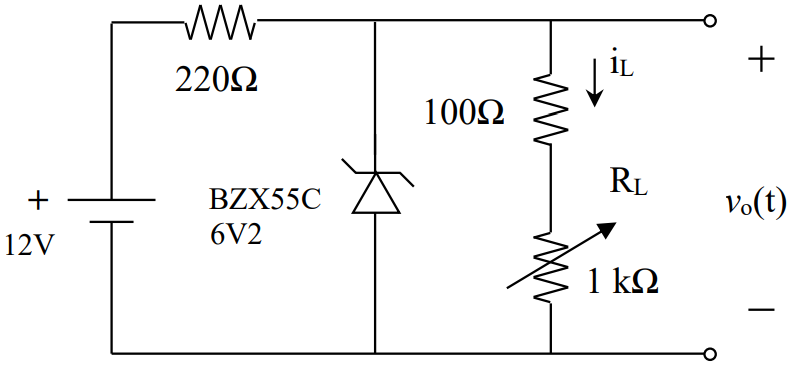
\includegraphics[width=1\textwidth]{10_1.png}
   \caption{Regulation with zener diode circuit schematic for the Step 10}
\end{figure} 
Then , the circuit given in Figure 23 is set in LTSpice environment.
\begin{figure}[H]
    \centering
   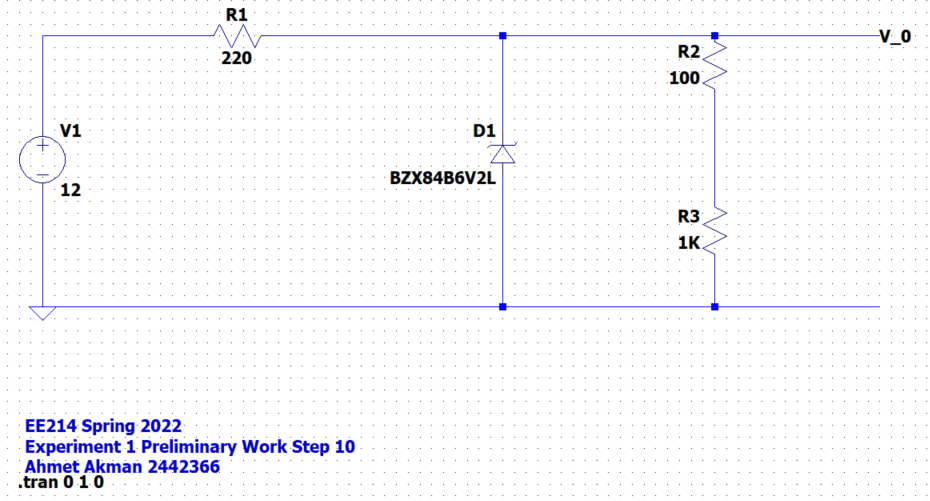
\includegraphics[width=1\textwidth]{10SCH.png}
   \caption{Regulation with zener diode circuit simulation schematic for the Step 10}
\end{figure} 

As the result it can be said that the \(v_o\) takes the minimum value of 6.217 Volts and maximumn of 6.221 Volts.
\section{Step 11}
%LTSpice
The clipper circuit given in Figure 24 is considered. 
\begin{figure}[H]
    \centering
   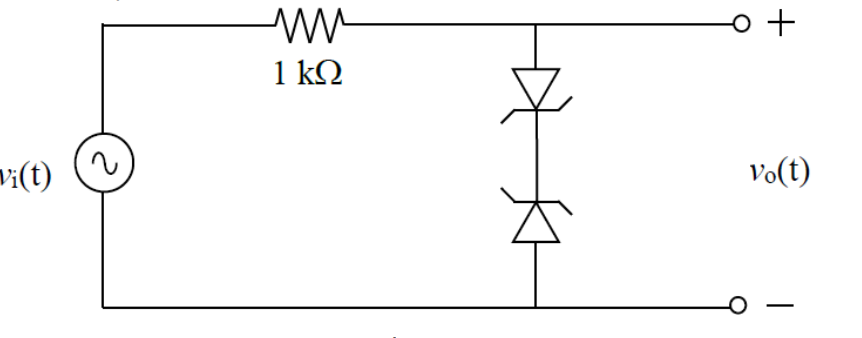
\includegraphics[width=1\textwidth]{11_1.png}
   \caption{Clipper circuit schematic for the Step 11}
\end{figure} 
The circuit given in Figure 25 is constructed in LTSpice environment.

\begin{figure}[H]
\centering
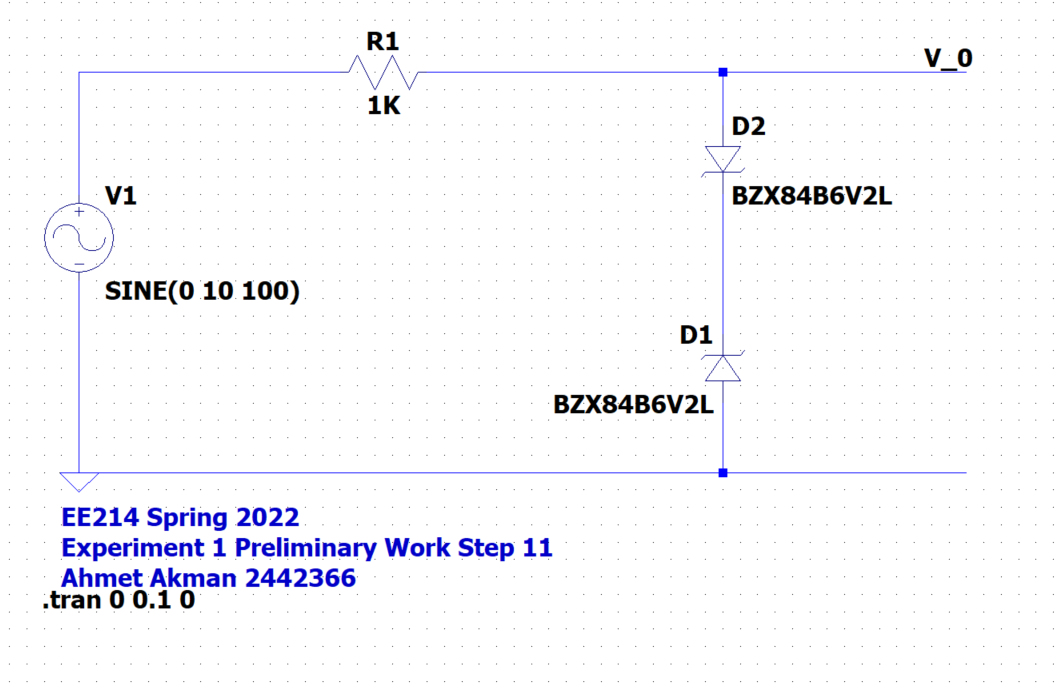
\includegraphics[width=1\textwidth]{11SCH.png}
\caption{Clipper circuit simulation schematic for the Step 11}
\end{figure} 

As the result the plot given in Figure 26 is obtained.

\begin{figure}[H]
    \centering
   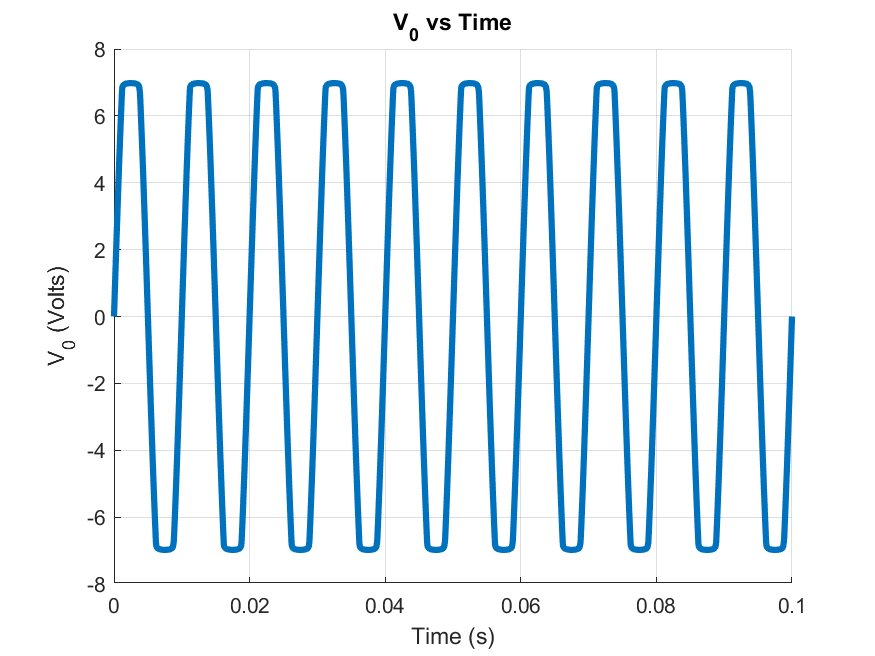
\includegraphics[width=1\textwidth]{11.png}
   \caption{Clipper circuit simulation plot \(V_o\) }
\end{figure} 
It can be said that the circuit clips the peaks of the input.
\iffalse
\section{Step 12}
%LTSpice and BONUS

\subsection{a)}
\begin{figure}[H]
    \centering
   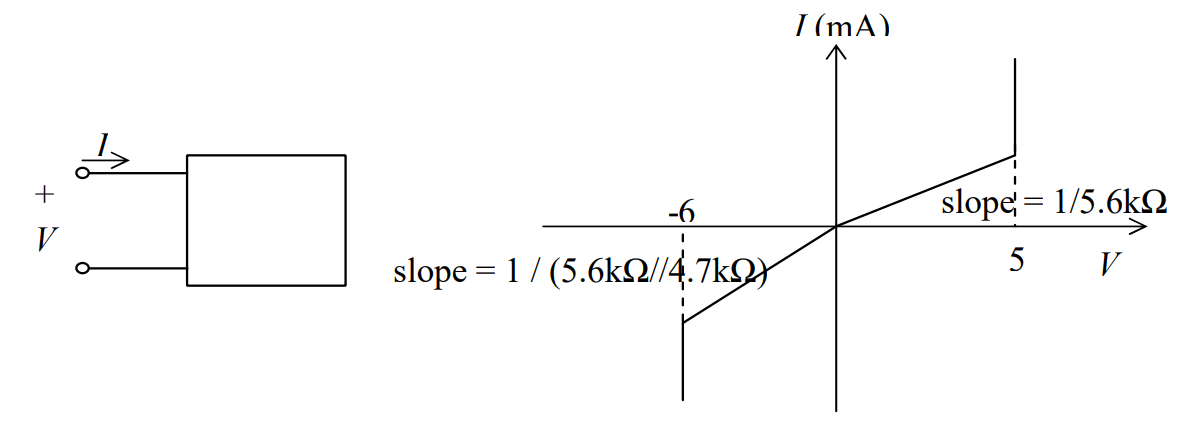
\includegraphics[width=1\textwidth]{12_1.png}
   \caption{i-v characteristics of a box for the Step 12 part a}
\end{figure} 

\subsection{b)}
\begin{figure}[H]
    \centering
   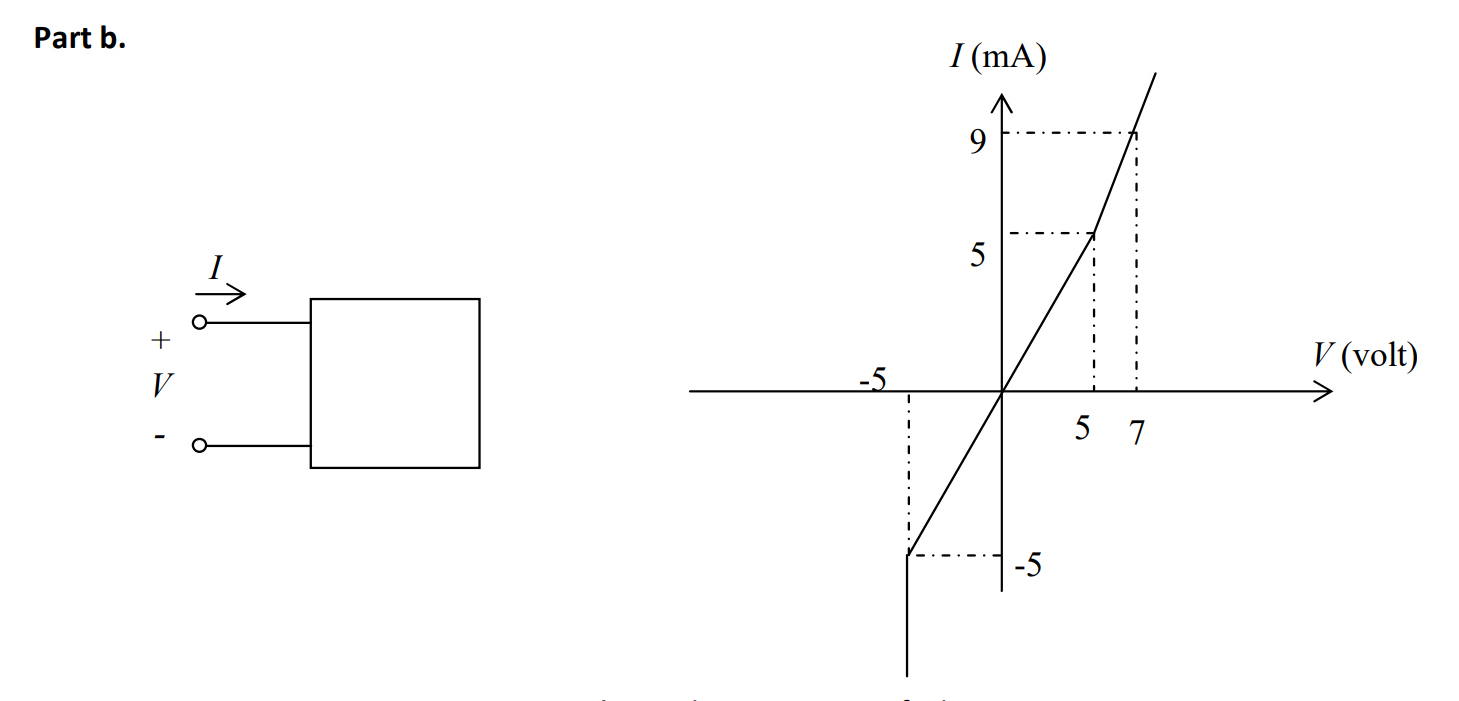
\includegraphics[width=1\textwidth]{12_2.png}
   \caption{i-v characteristics of a box for the Step 12 part b}
\end{figure} 
\fi
\section{Conclusion}
In conclusion, as the preliminary work of the first experiment. Some of the rectifier circuts with different diodes are investigated. In this way, various simulations are made. Different kinds of analysis' are done. Therefore their resutls are plotted.
\section*{Appendix A}
The results of the simulations are fetched from LTSpice and plotted in MATLAB in order to make the plots more readable and convinient.
\section*{Appendix B} \label{AB}
Figure 27 stands for no capacitor setup.
\begin{figure}[H]
    \centering
   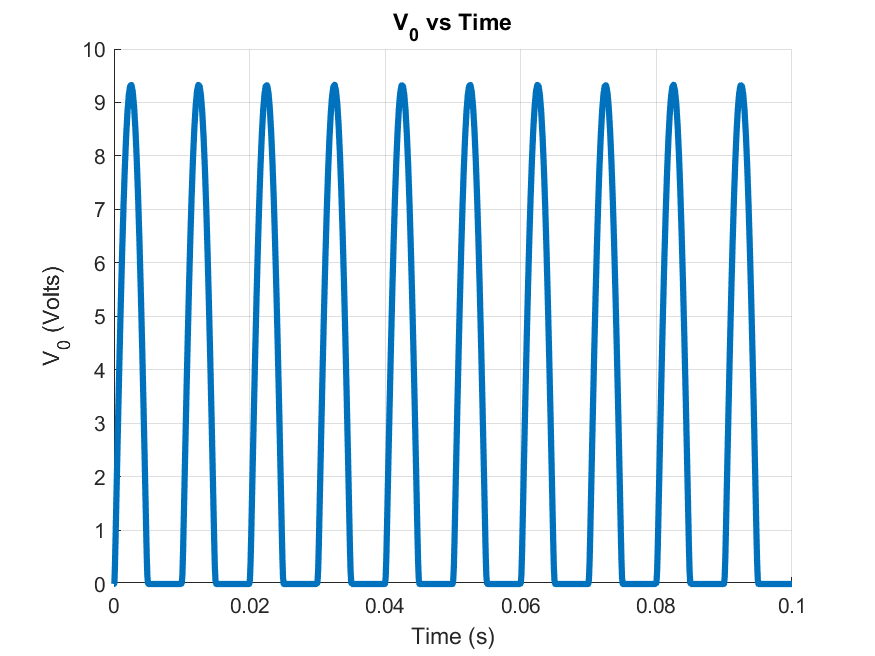
\includegraphics[width=1\textwidth]{6_0F.png}
   \caption{Half wave rectifier circuit simulation plot no capacitor \(V_o\) }
\end{figure} 

Figure 28 stands for 10nF capacitor setup.
\begin{figure}[H]
    \centering
   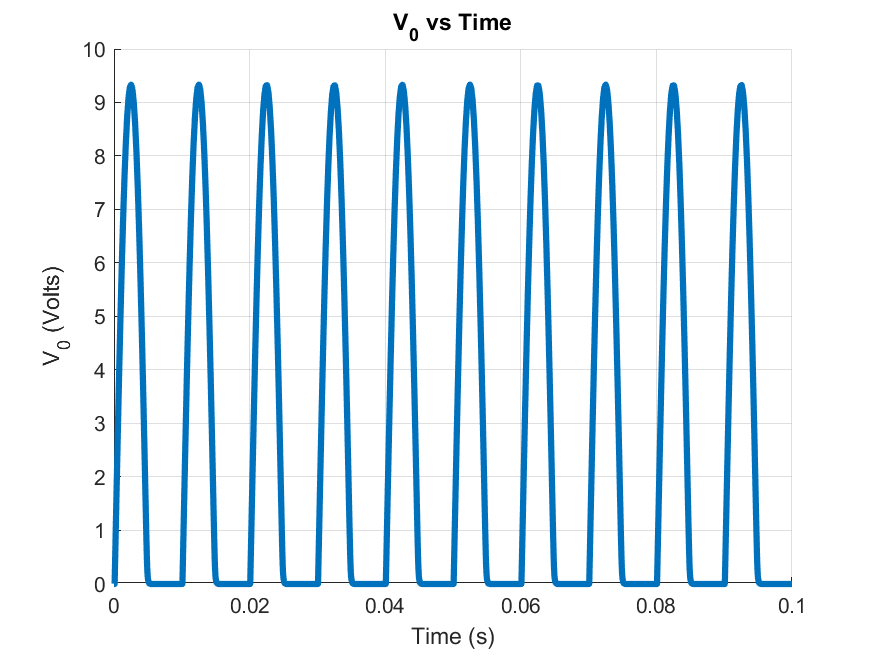
\includegraphics[width=1\textwidth]{6_10nF.png}
   \caption{Half wave rectifier circuit simulation plot 10nF capacitor \(V_o\) }
\end{figure} 
Figure 29 stands for 1uF capacitor setup.
\begin{figure}[H]
    \centering
   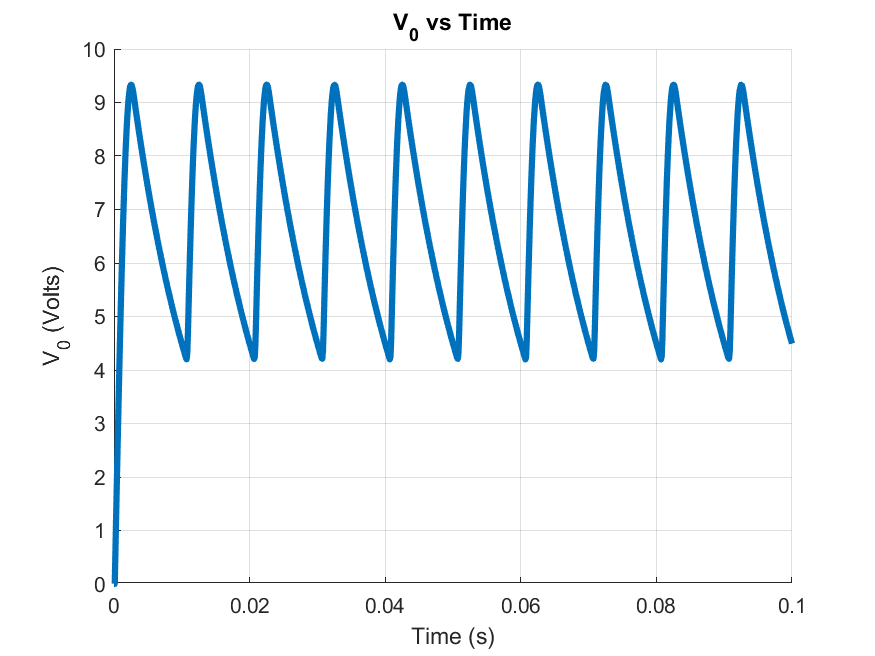
\includegraphics[width=1\textwidth]{6_1uF.png}
   \caption{Half wave rectifier circuit simulation plot 1uF \(V_o\) }
\end{figure} 

\end{document}

%%%%%%%%%%%%%%%%%%%%%%   EXAMPLE TABLE   %%%%%%%%%%%%%%%%%%%%%%%%%%%%%%%%
\begin{table}[H]
\begin{center}
    \caption{Resistance reading by color code convention.}
    \vspace{2mm}
    \begin{tabular}{||c | c | c||} 
        \hline
        Color Order & Value & Tolerance \\ [0.5ex] 
        \hline\hline
        Brown / Black / Red / Gold & 1k\( \Omega \) & \( \% \) 5  \\ 
        \hline
        Yellow / Violet / Red / Gold & 4.7k\( \Omega \) & \( \% \) 5   \\
        \hline
        Brown / Grey / Orange / Gold & 18k\( \Omega \) & \( \% \) 5  \\ [1ex] 
        \hline
    \end{tabular}
\end{center}
\end{table}


%%%%%%%%%%%%%%%%%%%%%%   EXAMPLE IMAGE   %%%%%%%%%%%%%%%%%%%%%%%%%%%%%%%%
\begin{figure}[H]
\centering
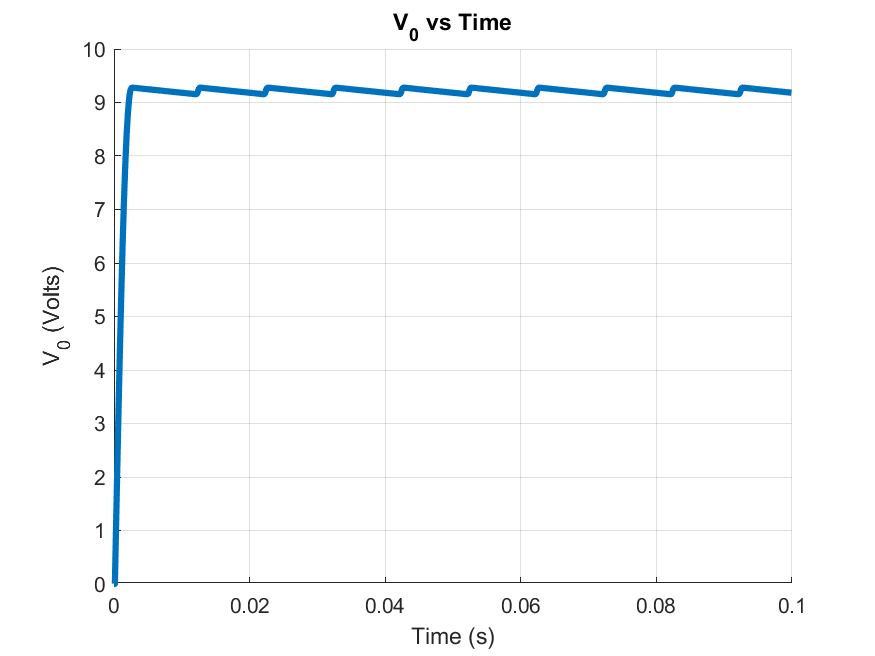
\includegraphics[width=1\textwidth]{5.png}
\caption{Circuit schematic for the step 5}
\end{figure} 

%%%%%%%%%%%%%%%%%%%%%%   EXAMPLE IMAGE FROM PDF   %%%%%%%%%%%%%%%%%%%%%%%%%%%%%%%%
\begin{figure}[H] \centering{
	\includegraphics[scale=0.25]{2a_plot.pdf}}
	\caption{Experiment 2}
\end{figure}
	